\documentclass{beamer}
%\documentclass[11pt,aspectratio=43]{beamer}% default
%\documentclass[11pt,aspectratio=169]{beamer}% test
\usetheme{NRLpresentation}

\titlegraphic{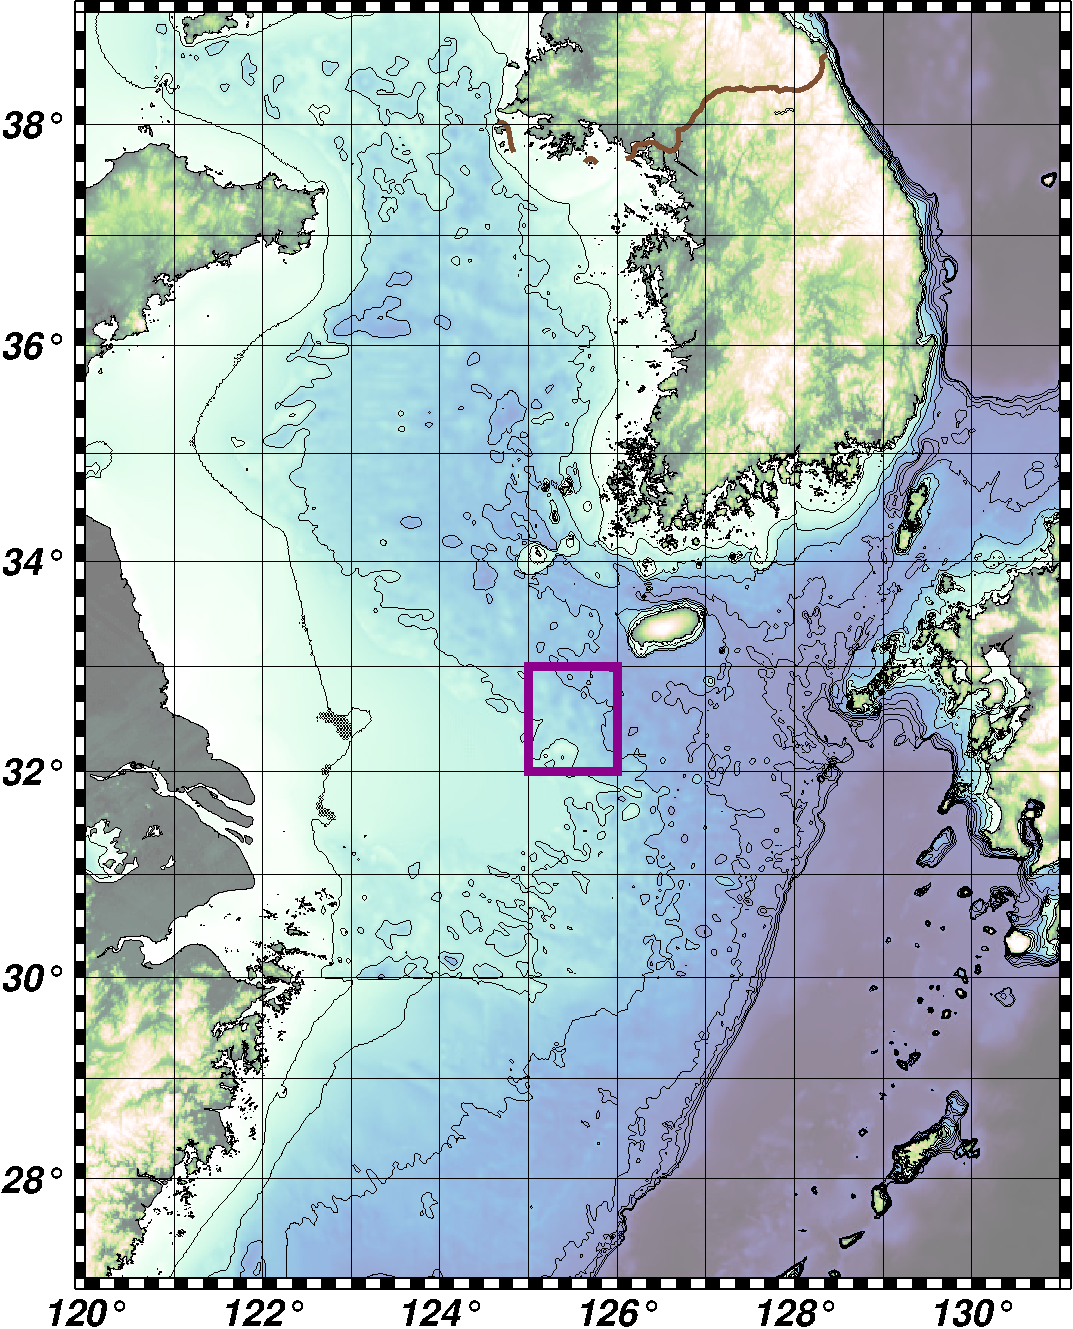
\includegraphics[width=0.9\textwidth]{TAVEX-overview-3}}% optional

\title{A \LaTeX\ Beamer Theme for\\ N.R.L.\ Presentations}
%\subtitle{Work Supported by the U.S. Office of Naval Research}% optional

\author{Peter Mignerey}

\institute{U.S. Naval Research Laboratory\\Acoustics Division, Washington DC}

\date{\today}

%\NRLcredit{Work Supported by the U.S. Office of Naval Research}% optional
%\NRLmark{SAMPLE // CLASSIFICATION}% optional
%\NRLpatents{Example Patents\\7,749,438 and 7,754,145}% optional
%\NRLdist{Distribution statement}% optional

\begin{document}

\begin{frame}
  \titlepage
\end{frame}

\begin{frame}
  \frametitle{Table of Contents}
  \tableofcontents
\end{frame}

\section{N.R.L.\ Beamer Theme}

\begin{frame}
  \frametitle{Introduction}
  This package provides a \LaTeX\ Beamer theme for presentations that mimic the N.R.L.\ corporate presentation style.
  \\\vspace{1em}
  Historically, Microsoft Word and PowerPoint have been limited in their support for integrating equations with text.
  %MathType alleviated the difficulty somethat, but is now broken on Macs, allegedly for computer security reasons.
  MathType alleviates the problem somethat, but the basic difficulty of seamlessly integrating equations with text remains.
  For those of us who write papers and presentations that include extensive mathematics, 
  this situation is a problem that many of us have resolved by turning to \LaTeX.
  With Beamer, one can simply cut text and equations from a paper and paste them into a presentation --- or conversely.
\end{frame}

\begin{frame}
  \frametitle{Installation}
  After unzipping the package, either place all files in a directory where you are preparing a talk, or more properly in the \LaTeX\ search path on your computer:
  \begin{description}
  \item[Linux] {\tt \$HOME/texmf/tex/latex/NRLpresentation}
  \item[Mac OS X] {\tt \$HOME/Library/texmf/tex/latex/NRLpresentation}
  \item[Windows] {\tt \%USERPROFILE\%\textbackslash{texmf}\textbackslash{tex}\textbackslash{latex}\textbackslash{NRLpresentation}}
  \end{description}
  TexLive and MacTex know about these default directories, and nothing further need be done.  
  Some other \LaTeX\ distributions may require running {\bf texhash} to rebuild a table of directories containing all of the style packages.
\end{frame}

\begin{frame}[fragile]
  \frametitle{Synopsis}
\footnotesize
\begin{verbatim}
\documentclass{beamer}
\usetheme{NRLpresentation}
\title{...}
\subtitle{...} % optional
\author{...}
\institute{U.S. Naval Research Laboratory\\
  Acoustics Division, Washington DC}
\date{\today}
\NRLcredit{Work Supported by ...} % optional
\NRLpatents{...} % optional list of patents
\NRLdist{...} % optional distribution statement
\NRLmark{MARK} % optional security marking
\titlegraphic{\includegraphics{magnificant-image}} % optional
\begin{document}
\begin{ frame }
...
\end{ frame }
\end{document}
\end{verbatim}
\end{frame}

\begin{frame}
  \frametitle{Beamer Class Options}
  \begin{description}
  \item[syntax] {\tt \textbackslash documentclass$\left[\mathtt{option}, \mathtt{option}=value,\ldots\right]$\{beamer\}}
  \item
  \item[font size] [ 8pt, 9pt, 10pt, 11pt (default), 12pt, 14pt, 17pt, 20pt ]
  \item[aspectratio=] [ 1610, 169, 149, 54, 43 (default), 32 ]\\
    \hspace{2.5pt}produces ratios: 16:10, 16:9, 14:9, 5:4, 4:3, 3:2\\ \vspace*{1ex}
  \end{description}
  \begin{itemize}
  \item These options are useful for fitting your talk within slides.
  \item Aspect ratio enables you to match a projector-screen shape.
    \begin{itemize}
    \item Keep in mind that a layout designed for one ratio may not fit another without adjustment.
    \end{itemize}
  \item Font size is a relative number.
    \begin{itemize}
    \item It also scales slide titles.
    \item The 11pt default is large, as seen in this documentation.
    \end{itemize}
  \end{itemize}
\end{frame}

\begin{frame}
  \frametitle{NRL Presentation Options}
  \framesubtitle{part I}
  \begin{description}
  \item[syntax] {\tt \textbackslash usetheme$\left[\mathtt{option}=value,\ldots\right]$\{NRLpresentation\}}
  \item
  \item[titlepage=] choose a format for the title page
    \begin{description}
    \item[corporate] (default) 
    \item[graphic] use with a {\tt titlegraphic}
    \item[classic] similar to Beamer default theme
    \end{description}
  \item[titlecolor=] choose background color of title page and slide heads
    \begin{description}
    \item[facets] (default) with white text
    \item[blue] with white text
    \item[white] with black text
    \end{description}
  \item[pagecolor=] choose the background color of slides
    \begin{description}
    \item[white] (default) with black text
    \item[blue] with white text
    \item[navy] with white text
    \end{description}
  \end{description}
\end{frame}

\begin{frame}
  \frametitle{NRL Presentation Options}
  \framesubtitle{part II}
  \begin{description}
  \item[bullets=] choose the type of bullets you prefer
    \vspace*{-1em}
    \begin{columns}[t]
      \begin{column}{0.06\textwidth}
        % dummy column that shoves the other two toward the right
      \end{column}
      \begin{column}{0.31\textwidth}
        \begin{description}
        \item[dotdash] (default) 
        \item[mixed] 
        \item[dashes] 
        \end{description}
      \end{column}
      \begin{column}{0.20\textwidth}
        \begin{description}
        \item[]
        \item[triangles] 
        \item[squares] 
        \end{description}
      \end{column}
      \begin{column}{0.20\textwidth}
        \begin{description}
        \item[]
        \item[balls] 
        \item[circles] 
        \end{description}
      \end{column}
    \end{columns}
  \vspace*{1ex}
  \item[underline=] choose whether to underline slide titles
    \begin{description}
    \item[false] (default) 
    \item[true]
    \end{description}
  \item[navigation=] choose whether to show the Beamer navigation bar
    \begin{description}
    \item[false] (default) 
    \item[true] 
    \end{description}
  \end{description}
\end{frame}

\begin{frame}
  \frametitle{N.R.L.\ Preamble Options}
  The following optional commands print properly formatted N.R.L.--specific information on the title page.
  \vspace{1em}
  \begin{description}
  \item[NRLcredit] \{sponsor recognition\}
  \item[NRLpatents] \{list of patents\}
  \item[NRLdist] \{distribution statement\}
  \item[NRLmark] \{MARK\} page classification mark
  \end{description}
\end{frame}

\section{Examples}

\NRLcredit{Work Supported by the U.S. Office of Naval Research}% optional
\NRLpatents{Example Patents\\7,749,438 and 7,754,145}% optional
\NRLdist{Any distribution statement will show up here.}
\NRLmark{SAMPLE // CLASSIFICATION}% optional

% The following undocumented functions are not normally needed 
% because they are automatically invoked by the NRLpresentation theme options.
% They are only used here to switch among various themes for illustration purposes.
% With them you can put multiple talks with different styles into one tex file.
% NRLtitleFunc, NRLtitleCorporateFunc, NRLtitleGraphicFunc, NRLtitleClassicFunc, 
% NRLtitlecolorFacets, NRLtitlecolorBlue, NRLtitlecolorWhite, 
% NRLpagecolorWhite, NRLpagecolorBlue, NRLpagecolorNavy, 
% NRLframeFunc, NRLframePlainTitleFunc, NRLframeUnderlineTitleFunc, 
% NRLbulletsDotdash, NRLbulletsMixed, NRLbulletsDashes, 
% NRLbulletsTriangles, NRLbulletsSquares, NRLbulletsBalls, NRLbulletsCircles

% show titlepage formats
\subsection{Title-Page Formats}
\NRLtitleFunc{\NRLtitleCorporateFunc}
\NRLtitlecolorFacets
\subtitle{[ titlepage = corporate ] (default)}
\begin{frame}
  \titlepage
\end{frame}

\NRLtitleFunc{\NRLtitleGraphicFunc}
\NRLtitlecolorFacets
\subtitle{[ titlepage = graphic ]}
\begin{frame}
  \titlepage
\end{frame}

\NRLtitleFunc{\NRLtitleClassicFunc}
\NRLtitlecolorFacets
\subtitle{[ titlepage = classic ]}
\begin{frame}
  \titlepage
\end{frame}

% show titlepage colors
\subsection{Title-Page Colors}
\NRLtitleFunc{\NRLtitleCorporateFunc}
\NRLtitlecolorFacets
\subtitle{[ titlecolor = facets ] (default)}
\begin{frame}
  \titlepage
\end{frame}

\NRLtitleFunc{\NRLtitleCorporateFunc}
\NRLtitlecolorBlue
\subtitle{[ titlecolor = blue ]}
\begin{frame}
  \titlepage
\end{frame}

\NRLtitleFunc{\NRLtitleCorporateFunc}
\NRLtitlecolorWhite
\subtitle{[ titlecolor = white ]}
\begin{frame}
  \titlepage
\end{frame}

% show page colors
\NRLtitlecolorFacets
\NRLpagecolorWhite
\subsection{Page Colors}
\begin{frame}
  \frametitle{Pagecolor}
  \framesubtitle{[ pagecolor = white ] (default)}
  Beamer has only three levels of bullets.
  When a slide comprises only a list, the outermost level should be a {\bf block} environment,
  which effectively provides a fourth level.
  \begin{block}{[ bullets = dotdash ]}
    \begin{itemize}
    \item Level 1
      \begin{itemize}
      \item Level 2
        \begin{itemize}
        \item Level 3
        \end{itemize}
      \end{itemize}
    \end{itemize}
  \end{block}
\end{frame}

\NRLtitlecolorFacets
\NRLpagecolorBlue
\NRLframeFunc{\NRLframePlainTitleFunc}
\begin{frame}
  \frametitle{Pagecolor}
  \framesubtitle{[ pagecolor = blue ]}
  Beamer has only three levels of bullets.
  When a slide comprises only a list, the outermost level should be a {\bf block} environment,
  which effectively provides a fourth level.
  \begin{block}{[ bullets = dotdash ]}
    \begin{itemize}
    \item Level 1
      \begin{itemize}
      \item Level 2
        \begin{itemize}
        \item Level 3
        \end{itemize}
      \end{itemize}
    \end{itemize}
  \end{block}
\end{frame}

\NRLtitlecolorFacets
\NRLpagecolorNavy
\NRLframeFunc{\NRLframePlainTitleFunc}
\begin{frame}
  \frametitle{Pagecolor}
  \framesubtitle{[ pagecolor = navy ]}
  Beamer has only three levels of bullets.
  When a slide comprises only a list, the outermost level should be a {\bf block} environment,
  which effectively provides a fourth level.
  \begin{block}{[ bullets = dotdash ]}
    \begin{itemize}
    \item Level 1
      \begin{itemize}
      \item Level 2
        \begin{itemize}
        \item Level 3
        \end{itemize}
      \end{itemize}
    \end{itemize}
  \end{block}
\end{frame}

% show underline
\subsection{Underlined Titles}

\NRLtitlecolorFacets
\NRLpagecolorBlue
\NRLframeFunc{\NRLframeUnderlineTitleFunc}
\begin{frame}
  \frametitle{Pagecolor}
  \framesubtitle{[ titlecolor = facets, pagecolor = blue, underline = true ]}
  An underlined slide title is nice when the title and page colors are the same.\\
  \vspace{1em}
  Beamer has only three levels of bullets.
  When a slide comprises only a list, the outermost level should be a {\bf block} environment,
  which effectively provides a fourth level.
  \begin{block}{[ bullets = dotdash ]}
    \begin{itemize}
    \item Level 1
      \begin{itemize}
      \item Level 2
        \begin{itemize}
        \item Level 3
        \end{itemize}
      \end{itemize}
    \end{itemize}
  \end{block}
\end{frame}

\NRLtitlecolorWhite
\NRLpagecolorWhite
\NRLframeFunc{\NRLframeUnderlineTitleFunc}
\begin{frame}
  \frametitle{Pagecolor}
  \framesubtitle{[ titlecolor = white, pagecolor = white, underline = true ]}
  A white page with black type is useful for printing drafts and handouts.\\
  \vspace{1em}
  Beamer has only three levels of bullets.
  When a slide comprises only a list, the outermost level should be a {\bf block} environment,
  which effectively provides a fourth level.
  \begin{block}{[ bullets = dotdash ]}
    \begin{itemize}
    \item Level 1
      \begin{itemize}
      \item Level 2
        \begin{itemize}
        \item Level 3
        \end{itemize}
      \end{itemize}
    \end{itemize}
  \end{block}
\end{frame}

% show bullets
\NRLtitlecolorFacets
\NRLpagecolorWhite
\NRLframeFunc{\NRLframePlainTitleFunc}

\NRLmark{UNCLASSIFIED}

\section{Classification Marks}

\begin{frame}
  \frametitle{Page Marks}
  {\bf syntax} \quad {\tt \textbackslash{NRLmark}\{$\left<MARK\right>$\}}
  \vspace{1em}
  \begin{itemize}
  \item This command places classification marks at the top and bottom of each page.
  \item Typically placed in the preamble, it may be reissued between frames to change the marking.
  \item Both arguments are mandatory, but may be empty\ {\tt\{\}}.
  \item The marks may be resized or colored by modifying the arguments:
    {\tt\{\textbackslash{huge}\textbackslash{textcolor}\{red\}\{MARK\}\}}
  \end{itemize}
\end{frame}

\begin{frame}
  \frametitle{Paragraph Marks}
  Because paragraph marks must be typed so frequently, some quickly typed shortcuts are provided for a few common markings.
  \vspace{1em}
  \begin{NRLtable}{}{List of Paragraph Marking Commands}
    \begin{tabular}{|l|l|}
      \hline
      COMMAND\hspace{1in} 	& PRODUCES\\
      \hline\hline
          {\tt \textbackslash u} & {(U)}\\
          {\tt \textbackslash uf} & {(U//FOUO)}\\
          {\tt \textbackslash c} & {(C)}\\
          {\tt \textbackslash s} & {(S)}\\
          {\tt \textbackslash sn} & {(S//NF)}\\
          \hline
    \end{tabular}
  \end{NRLtable}
\end{frame}

\NRLmark{}

\section{Bullets}

\begin{frame}
  \frametitle{Bullets}
  Beamer has only three levels of bullets.
  When a slide comprises only a list, the outermost level should be a {\bf block} environment,
  which effectively provides a fourth level.
  \NRLbulletsDotdash
  \begin{block}{[ bullets = dotdash ] (default)}
    \begin{itemize}
    \item Level 1
      \begin{itemize}
      \item Level 2
        \begin{itemize}
        \item Level 3
        \end{itemize}
      \end{itemize}
    \end{itemize}
  \end{block}
\end{frame}

\begin{frame}
  \frametitle{Bullets}
  \NRLbulletsMixed
  \begin{block}{[ bullets = mixed ]}
    \begin{itemize}
    \item Level 1
      \begin{itemize}
      \item Level 2
        \begin{itemize}
        \item Level 3
        \end{itemize}
      \end{itemize}
    \end{itemize}
  \end{block}
  \NRLbulletsDashes
  \begin{block}{[ bullets = dashes ]}
    \begin{itemize}
    \item Level 1
      \begin{itemize}
      \item Level 2
        \begin{itemize}
        \item Level 3
        \end{itemize}
      \end{itemize}
    \end{itemize}
  \end{block}
\end{frame}

\begin{frame}
  \frametitle{Bullets}
  \NRLbulletsTriangles
  \begin{block}{[ bullets = triangles ]}
    \begin{itemize}
    \item Level 1
      \begin{itemize}
      \item Level 2
        \begin{itemize}
        \item Level 3
        \end{itemize}
      \end{itemize}
    \end{itemize}
  \end{block}
  \NRLbulletsSquares
  \begin{block}{[ bullets = squares ]}
    \begin{itemize}
    \item Level 1
      \begin{itemize}
      \item Level 2
        \begin{itemize}
        \item Level 3
        \end{itemize}
      \end{itemize}
    \end{itemize}
  \end{block}
\end{frame}

\begin{frame}
  \frametitle{Bullets}
  \NRLbulletsBalls
  \begin{block}{[ bullets = balls ]}
    \begin{itemize}
    \item Level 1
      \begin{itemize}
      \item Level 2
        \begin{itemize}
        \item Level 3
        \end{itemize}
      \end{itemize}
    \end{itemize}
  \end{block}
  \NRLbulletsCircles
  \begin{block}{[ bullets = circles ]}
    \begin{itemize}
    \item Level 1
      \begin{itemize}
      \item Level 2
        \begin{itemize}
        \item Level 3
        \end{itemize}
      \end{itemize}
    \end{itemize}
  \end{block}
\end{frame}

\section{Figures \& Tables}

\subsection{Figures}

\begin{frame}[fragile]
  \frametitle{N.R.L.\ Figure Syntax}
  {\bf syntax} \quad {\tt \textbackslash begin\{NRLfigure\}\{$\left<mark\right>$\}\{$\left<title\right>$\}\{$\left<caption\right>$\}}
  \small
  \begin{itemize}
  \item All three arguments are mandatory, but may be empty\ {\tt\{\}}.
  \item No frame is printed when the mark is empty.
  \item The mark, title \& caption may be resized or colored by modifying the arguments:
    {\tt\{\textbackslash{huge}\textbackslash{textcolor}\{red\}\{MARK\}\}}
  \item Hyphenation is suppressed within captions.
  \item Line breaks {(\textbackslash\textbackslash)} do not work within captions.
  \end{itemize}
\vspace{1em}
{\bf example}
\footnotesize
\begin{verbatim}
  \begin{NRLfigure}{UNCLASSIFIED}{TITLE}{CAPTION}
    
\includegraphics[width=0.4\columnwidth]{NRL-Navy-Seal}%
  \end{NRLfigure}
\end{verbatim}
\end{frame}

\begin{frame}
  \frametitle{Standard {\LaTeX} Figure}
  \begin{figure}
    
\includegraphics[width=0.4\columnwidth]{NRL-Navy-Seal}
    \caption{For a standard LaTeX figure, captions are ragged right within the full width of a slide, and are set in the normal size font. The quick brown fox jumped over the lazy dog. The quick brown fox jumped.}
  \end{figure}
\end{frame}

\begin{frame}
  \frametitle{N.R.L.\ Figure}
  \begin{NRLfigure}{}{OPTIONAL TITLE}{For an N.R.L.\ figure, captions span the figure width down to a minimum size, and are set in footnote size font. Also, an optional title is provided.}
    
\includegraphics[width=0.4\columnwidth]{NRL-Navy-Seal}%
  \end{NRLfigure}
\end{frame}

\NRLmark{UNCLASSIFIED}

\begin{frame}
  \frametitle{N.R.L.\ Figure}
  \framesubtitle{boxed with markings}
  \begin{NRLfigure}{UNCLASSIFIED}{\u TITLE}{\u Short captions are centered.}
    
\includegraphics[width=0.4\columnwidth]{NRL-Navy-Seal}%
  \end{NRLfigure}
\end{frame}

\NRLmark{}

\subsection{Tables}

\begin{frame}[fragile]
  \frametitle{N.R.L.\ Table Syntax}
  \framesubtitle{simple table}
  {\bf syntax} \quad {\tt \textbackslash begin\{NRLtable\}\{$\left<mark\right>$\}\{$\left<caption\right>$\}}\\
  \begin{itemize}
  \item Both arguments are mandatory, but may be empty {\tt\{\}}.
  \item The mark \& caption may be resized or colored.
  \item Line breaks {(\textbackslash\textbackslash)} do not work within captions.
  \item Table elements and notes may be resized either individually or as a group.
  \end{itemize}
{\bf example}
\tiny
\begin{verbatim}
\begin{NRLtable}{}{Table caption.}
  \begin{tabular}{|l|c|c|c|c|} \hline
    & Day 1 & Day 2 & Day 3 & Day 4 \\ \hline
    Start Time (day)	& 347.75 & 350.50 & 353.50 & 357.80 \\
    End Time (day)	& 348.75 & 351.50 & 354.50 & 358.80 \\ \hline
    300 Hz SNR (dB)	& 28.7 & 31.5 & 26.3 & 26.0 \\
    500 Hz SNR (dB)	& 18.6 & 20.5 & 18.5 & 17.0 \\ \hline
    Wave Height (m)	& 1.7 & 2.0 & 2.1 & 1.5 \\
    Wind Speed (m/s)	& 7.8 & 6.7 & 7.1 & 6.5 \\ \hline
  \end{tabular}
\end{NRLtable}
\end{verbatim}
\end{frame}

\begin{frame}[fragile]
  \frametitle{N.R.L.\ Table Syntax}
  \framesubtitle{annotated table}
{\bf example}
  \tiny
\begin{verbatim}
\begin{NRLtable}{}{Table Caption}
  %\normalsize % optionally resize table elements here
  \begin{tabular}{|l|c|c|c|c|} \hline
    & Day 1 & Day 2 & Day 3 & Day 4 \\ \hline
    Start Time (day)\tnote	& 347.75 & 350.50 & 353.50 & 357.80 \\
    End Time (day)\tnote{a}	& 348.75 & 351.50 & 354.50 & 358.80 \\ \hline
    300 Hz SNR (dB)		& 28.7 & 31.5 & 26.3 & 26.0 \\
    500 Hz SNR (dB)		& 18.6 & 20.5 & 18.5 & 17.0 \\ \hline
    Wave Height (m)\tnote	& 1.7 & 2.0 & 2.1 & 1.5 \\
    Wind Speed (m/s)\tnote{b}	& 7.8 & 6.7 & 7.1 & 6.5 \\ \hline
  \end{tabular}
  \begin{tablenotes}
    %\footnotesize % optionally resize table notes here
    \item The start and end times are fractional days within year 2003.
    \item The wave height and wind speed were acquired by NOAA-NDBC buoy 44004.
    \note Unnumbered additional comments like this are also supported.
    \noteN Numbered additional comments like this are also supported.
    \noteN Table notes are set in footnotesize.
  \end{tablenotes}
\end{NRLtable}
\end{verbatim}
\end{frame}

\begin{frame}
  \frametitle{Standard {\LaTeX} Table}
  \begin{table}
    \caption{For a standard LaTeX table, captions are ragged right within the full width of a slide, and are set in the normal size font. The quick brown fox jumped over the lazy dog. The quick brown fox jumped.}
    \begin{tabular}{|l|c|c|c|c|} \hline
      & Day 1 & Day 2 & Day 3 & Day 4 \\ \hline
      Start Time (day)	& 347.75 & 350.50 & 353.50 & 357.80 \\
      End Time (day)	& 348.75 & 351.50 & 354.50 & 358.80 \\ \hline
      300 Hz SNR (dB)	& 28.7 & 31.5 & 26.3 & 26.0 \\
      500 Hz SNR (dB)	& 18.6 & 20.5 & 18.5 & 17.0 \\ \hline
      Wave Height (m)	& 1.7 & 2.0 & 2.1 & 1.5 \\
      Wind Speed (m/s)	& 7.8 & 6.7 & 7.1 & 6.5 \\ \hline
    \end{tabular}
  \end{table}
\end{frame}

\begin{frame}
\frametitle{N.R.L.\ Table}
\framesubtitle{a simple table}
\begin{NRLtable}{}{For an N.R.L.\ table, captions span the table width down to a minimum size, and are set in normal size font as are the table items. Hyphenation is suppressed.}
  \begin{tabular}{|l|c|c|c|c|} \hline
    & Day 1 & Day 2 & Day 3 & Day 4 \\ \hline
    Start Time (day)	& 347.75 & 350.50 & 353.50 & 357.80 \\
    End Time (day)	& 348.75 & 351.50 & 354.50 & 358.80 \\ \hline
    300 Hz SNR (dB)	& 28.7 & 31.5 & 26.3 & 26.0 \\
    500 Hz SNR (dB)	& 18.6 & 20.5 & 18.5 & 17.0 \\ \hline
    Wave Height (m)	& 1.7 & 2.0 & 2.1 & 1.5 \\
    Wind Speed (m/s)	& 7.8 & 6.7 & 7.1 & 6.5 \\ \hline
  \end{tabular}
\end{NRLtable}
\end{frame}

\NRLmark{UNCLASSIFIED}

\begin{frame}
\frametitle{N.R.L.\ Table}
\framesubtitle{a simple table with markings}
\begin{NRLtable}{UNCLASSIFIED}{\u Short captions are centered.}
  \begin{tabular}{|l|c|c|c|c|} \hline
    & Day 1 & Day 2 & Day 3 & Day 4 \\ \hline
    Start Time (day)	& 347.75 & 350.50 & 353.50 & 357.80 \\
    End Time (day)	& 348.75 & 351.50 & 354.50 & 358.80 \\ \hline
    300 Hz SNR (dB)	& 28.7 & 31.5 & 26.3 & 26.0 \\
    500 Hz SNR (dB)	& 18.6 & 20.5 & 18.5 & 17.0 \\ \hline
    Wave Height (m)	& 1.7 & 2.0 & 2.1 & 1.5 \\
    Wind Speed (m/s)	& 7.8 & 6.7 & 7.1 & 6.5 \\ \hline
  \end{tabular}
\end{NRLtable}
\end{frame}

\NRLmark{}

\begin{frame}
\frametitle{N.R.L.\ Table}
\framesubtitle{with annotations \& notes}
\begin{NRLtable}{}{The {\tt threeparttable} package is included within the {\tt NRLtable} environment to support the annotation of items.}
  %\normalsize % optionally  resize table elements here
  \begin{tabular}{|l|c|c|c|c|} \hline
    & Day 1 & Day 2 & Day 3 & Day 4 \\ \hline
    Start Time (day)\tnote	& 347.75 & 350.50 & 353.50 & 357.80 \\
    End Time (day)\tnote{a}	& 348.75 & 351.50 & 354.50 & 358.80 \\ \hline
    300 Hz SNR (dB)		& 28.7 & 31.5 & 26.3 & 26.0 \\
    500 Hz SNR (dB)		& 18.6 & 20.5 & 18.5 & 17.0 \\ \hline
    Wave Height (m)\tnote	& 1.7 & 2.0 & 2.1 & 1.5 \\
    Wind Speed (m/s)\tnote{b}	& 7.8 & 6.7 & 7.1 & 6.5 \\ \hline
  \end{tabular}
  \begin{tablenotes}
    %\footnotesize % optionally  resize table notes here
    \item The start and end times are fractional days within year 2003.
    \item The wave height and wind speed were acquired by NOAA-NDBC buoy 44004.
    \note Unnumbered additional comments like this are also supported.
    \noteN Numbered additional comments like this are also supported.
    \noteN The default font size for table notes is {\tt footnotesize}.
  \end{tablenotes}
\end{NRLtable}
\end{frame}

\end{document}
